
In this section, we describe the currently discussed Provenance DM. We 
first explain the core elements with details for each class and relation (Section~\ref{sec:core_model}). We then define the extended model, introducing and defining specialized concepts and relation that brings useful provenance information for astronomy (Section~\ref{sec:extended_model}).

% 2018-09 commented for now
%An auto-generated documentation of all classes (VO-DML compliant) is available in the Volute repository at \url{https://volute.g-vo.org/svn/trunk/projects/dm/provenance/vo-dml/ProvenanceDM.html}.

% \subsection{Overview: Conceptional UML class diagram and introduction to core classes}
% \label{sec:overview}
%We give in this section an overview on the main classes. More details about 
%each class and their relations will be explained in the following sections.
%Its core elements are colored in blue. These core elements can also be found in the W3C Provenance Data
%Model. The pattern defined by these classes is very general and can be reused everywhere where provenance is needed. 

% \begin{figure}[ht]
% \centering
% 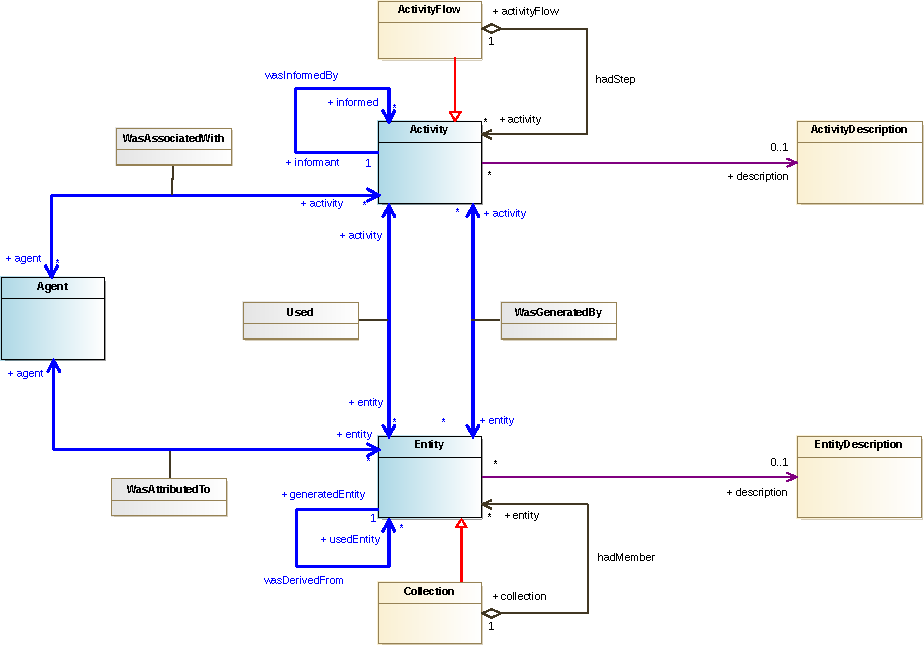
\includegraphics[width=1.0\textwidth]{domain-classdiagram-v2.pdf}
% \caption[Overview: conceptual class diagram of the Provenance Data
% Model]{Overview of the classes for the Provenance DM in a conceptual
% class diagram. The blue classes are core elements. There are a number of
% many-to-many relationships with attached association classes (grey) that may
% contain additional attributes.}
% %Objects in the blue box also appear in the W3C Provenance DM. 
% %Green classes are links to the IVOA Dataset Metadata Model.}
% \label{fig:classdiagram-conceptional}
% \end{figure}


%\label{sec:core}
% Some examples for different use cases are given in Section \ref{sec:usecases-implementations}.
% The elements of a provenance model can be expressed as a directed graph to capture the causal dependencies. 

%Figure~\ref{fig:classdiagram-conceptional} shows the conceptional UML diagram for an IVOA Provenance DM.


\subsection{Core Model}
\label{sec:core_model}

\subsubsection{Class diagram}

\begin{figure}[ht]
\centering
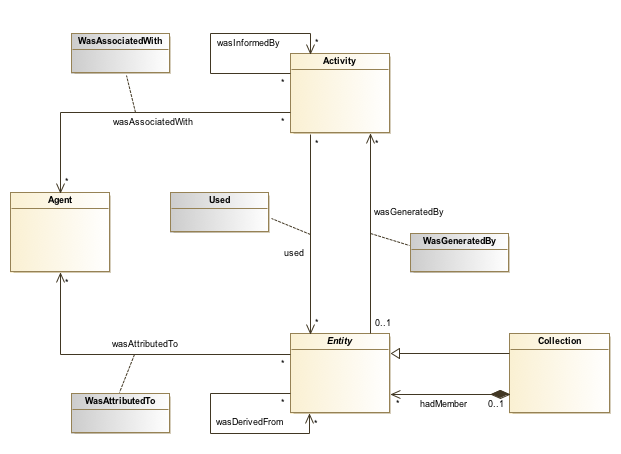
\includegraphics[width=1.0\textwidth]{CoreModel.png}
\caption[Core classes and relations of the Provenance DM]{The main core classes and relations of the Provenance DM, which are taken from the W3C PROV-DM.}
\label{fig:coreclasses}
\end{figure}

The core elements of the Provenance DM are \class{Entity},
\class{Activity} and \class{Agent}. For these elements, we chose the same names
that were used in the PROV recommendation of the World Wide Web Consortium
(W3C PROV, \citealt{std:W3CProvDM}), which defines a very abstract pattern that can
be reused here. The provenance information resides in the relations between those core elements, also taken from the W3C PROV-DM and the related ontology PROV-O \citealt{std:PROV-O}).

We present the core classes, along with their relations to each other, in
Figure~\ref{fig:coreclasses} and give short descriptions with some examples:

\begin{itemize}

\item \class{Entity:} a physical, digital, conceptual, or other kind of thing with some fixed aspects. For example: data products such as images, catalogs, parameter files,
calibration data, instrument characteristics, articles, web pages.

\item \class{Activity:} an action\slash{}process or a series of actions,
    occurring over a period of time, performed on or caused by entities,
    usually resulting in new entities. For example: data acquisition like
    observation, simulation; regridding, fusion, calibration steps,
    reconstruction; edition, publication, release of data.

\item \class{Agent:} executes\slash{}controls an activity, is responsible for
    an activity or an entity. For example: telescope astronomer, observatory, institute,
    pipeline operator, principal investigator, software engineer,
    project helpdesk.

\end{itemize}

\noindent


We use the following relation classes to specify the mapping between the three core  classes. The relation names were, again, chosen to match the W3C PROV-DM names:

\begin{itemize}

\item \class{wasGeneratedBy:} a new entity is generated by an activity\\
        (entity ``image.fits'' wasGeneratedBy activity ``observation'')

\item \class{used:} an entity is used by an activity\\
        (activity ``calibration'' used entities ``calibration data'', ``raw images'')

\item \class{wasAssociatedWith:} agents have responsibility for an activity\\
        (agent ``observer Max Smith'' wasAssociatedWith activity ``observation'')

\item \class{wasAttributedTo:} an entity can be attributed to an agent\\
        (entity ``image.fits'' wasAttributedTo ``observatory'')

\end{itemize}

% 2018-09 commented
% We showed the relations as extra classes (and thus boxes in the diagrams, instead of just having annotated relations), because they can have additional attributes -- when mapping the model to a relational database, these relations would appear as mapping tables.

The W3C PROV-DM and its related ontology PROV-O \citep{std:PROV-O} contain several components that are not described in this document. The IVOA Provenance DM having the same core concepts, it is possible to extend it with any W3C PROV component or extension. In addition, the ProvONE proposed extension to W3C PROV can be connected to this model in the context of scientific workflows.

%The W3C-model has the advantage of being already an approved standard, and it 
%contains all the necessary main features needed for a Provenance model for 
%Astronomy. However, it is very general, and by adding reusable prototypes, 
%templates or descriptions for activities and entities,  the model may fit better 
%to the astronomy domain.

% 2018-09 commented
%This separation into two classes may not be needed for each and every project,
%and everyone is free to choose which classes make sense for his\slash{}her use
%case. Also, when serializing provenance, one can integrate the description side into
%the other classes.
%%, thus producing a W3C compliant provenance description. 
%More details about all these classes and relations are given in the following
%section.


%It still remains to be seen if this separation into two classes is necessary, 
%useful or just nice to have. Currently, we include the descriptions in our model, 
%for normalization purposes. 

%But when serialising the provenance one could 
%integrate the description side into the other classes, thus producing W3C 
%compliant provenance.



\subsubsection{Entity}

\begin{table}[ht]
\small
\tymax  0.5\textwidth
\textbf{\normalsize Entity}\vspace{0.25em}\\
\begin{tabulary}{1.0\textwidth}{@{}lp{3.5cm}p{2cm}L@{}}
\toprule
\head{Attribute} & \head{W3C PROV} & \head{Data type} & \head{Description}\\
\midrule
\textbf{id} & prov:id & (qualified) string & a unique id for this entity (unique in its realm)\\
name       & prov:label & string & a human-readable name for the entity (to be displayed by clients)\\
location    & prov:location & string & a path or a geographical location, e.g. a URL\\
type        & prov:type  & string & a provenance type, i.e. one of: prov:collection, prov:bundle, prov:plan; or any of the specialized entities defined in Section~\ref{sec:spec_entities} \\
%description\_ref  & foreign key/url & link to \class{EntityDescription}\\
annotation  & prov:description & string & text describing the entity in more detail\\
value       & prov:value &  & provides a value that is a direct representation of an entity \\
creationTime  & prov:generatedAtTime & datetime & date and time at which the entity was created (e.g. timestamp of a file)\\
destructionTime  & prov:invalidatedAtTime & datetime & date and time at which the entity was erased or invalidated\\
rights      & -- & string & access rights for the entity, values: public, secure or proprietary; see Curation.Rights, RightsType in DatasetDM\\
%\midrule
%$\rightarrow$ description &  & link & link to \class{EntityDescription}\\
%$\rightarrow$ wasAttributedTo & prov:wasAttributedTo & link & link to \class{WasAttributedTo} for linking with a responsible \class{Agent}\\
\bottomrule
\end{tabulary}
\caption[Attributes of \class{Entities}]{Attributes of \class{Entities}. Mandatory attributes are marked in \textbf{bold}.
%, references are indicated with an arrow ($\rightarrow$). 
Further project-specific attributes (e.g. size, path, url, \dots) could be added when relevant for the project (see Section~\ref{sec:dataset-obscore}). 
% %mireille I would comment this here, because in the model they are in EntityDescrioption while in the implementation one can decide to gather attributes from Entity and EntityDescription together
%Attributes from \class{EntityDescription} (see next section) may appear here as well.
}\label{tab:entity}
\end{table}

Entities in astronomy are usually astronomical or astrophysical datasets in the 
form of images, tables, numbers, etc. But they can also be observation or 
simulation log files, files containing system information, environment
variables, names and versions of packages, ambient conditions, or, in a wider
sense, also observation proposals, scientific  articles, or manuals and other
documents. 

An entity is not restricted to being a file.
It can even be just a number in a table, depending on how fine-grained the 
provenance shall be described.
An entity can also carry its value directly in its \attribute{value} attribute.

%\begin{figure}[ht]
%\centering
%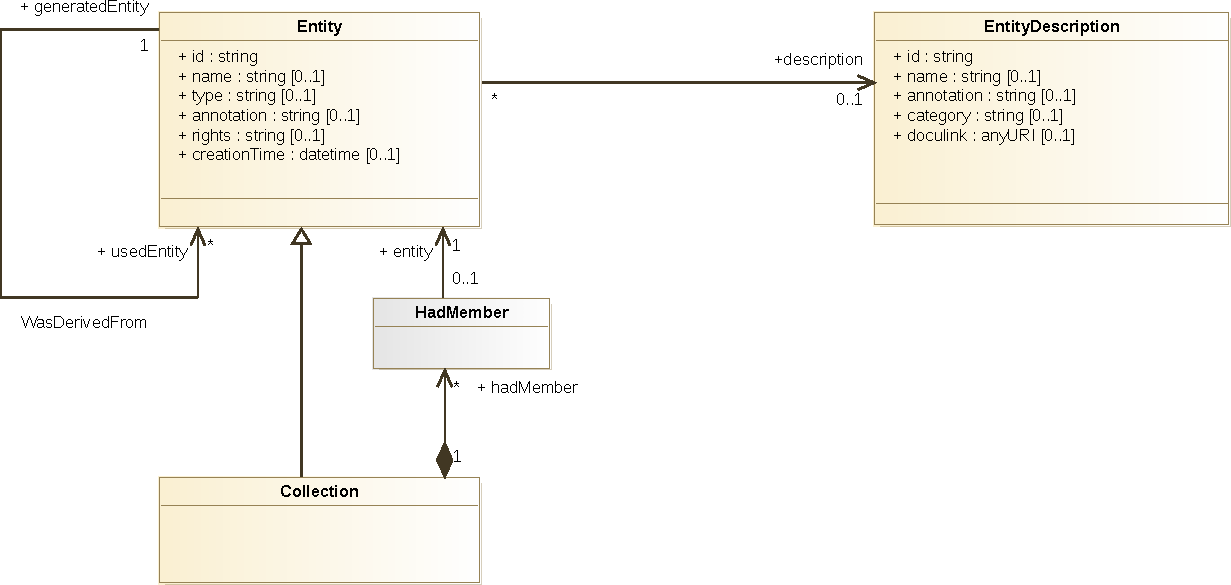
\includegraphics[scale=0.6]{entity-details-v2.pdf}
%\caption[Relations between Entity, EntityDescription and Collection]{The relations between Entity, %EntityDescription and Collection (see Section~\ref{sec:collection}). 
%Links to the Dataset class from the Dataset Metadata Model are described in Section~\ref{sec:dmlinks}.}
%\label{fig:entity-details}
%\end{figure}

The VO concept closest to \class{Entity} is the notion of \class{Dataset}, which
could mean a single table, an image or a collection of them. The Dataset
Metadata Model \citep{std:DatasetDM} specifies that a \class{Dataset} as ``a file or
files which  are considered to be a single deliverable''.  Most attributes of
the \class{Dataset} class can be mapped directly to attributes of the
\class{Entity} class, see the mappings of 
Table~\ref{tab:datasetmapping} in Section~\ref{sec:dmlinks}.

Entities have the attributes given in Table 
\ref{tab:entity}. If an attribute also exists in the W3C 
PROV-DM, we list its name in the second column.

%We discussed further attributes like \emph{size} and \emph{format}, but we decided to treat an
%entity of the same content but different format (and thus size) as the same entity,
%unless they do not have the same provenance (e.g. when the ``transformation'' activity
%for converting one format into another is included in the provenance description).

%\TODO{format and size may not be needed, if entities with the same content but different format and size are considered as the same entity.}

The difference between entities that are used as input data and those used as
output data becomes clear by specifying the relations between the data and the
activities producing or using these data. More details on this will follow in
Section \ref{sec:entity-activity-relations}.






\paragraph{WasDerivedFrom.}
%This relation, linking two entities together, is also borrowed from the W3C model. It is used to express that one entity was derived from another, e.g. it can be used to find one (or more) progenitor(s) of a dataset.
%, without having to look for the activities in between. It can therefore serve as a shortcut.

%The information this relation provides is somewhat redundant, since progenitors
%for entities can generally be found through the links to activity and the corresponding
%descriptions. Nevertheless, 
We include the \class{wasDerivedFrom} relation for those cases
where an explicit link between an entity and its progenitor(s) is useful. This relation infers the existence of an activity, but this activity may not be explicitly defined. Sub-classes of this relation in W3C PROV include the concepts of revisions and specializations \citep{std:W3CProvDM}.
%(e.g. for speeding up searches for  progenitors, or if the activity in between is not important).

Note that the \class{WasDerivedFrom} relation cannot always automatically be
inferred from following existing \class{WasGeneratedBy} and \class{Used} relations alone.
If there is more than one input and more than one output of an activity, it is
not clear which entity was derived from which. Only by specifying
the descriptions and roles accordingly, or by adding a \class{WasDerivedFrom}
relation, this direct derivation becomes known.


\begin{table}[ht]
\small
\tymax  0.5\textwidth
\textbf{\normalsize WasDerivedFrom}\vspace{0.25em}\\
\begin{tabulary}{1.0\textwidth}{@{}lp{3cm}L@{}}
\toprule
\head{Attribute} & \head{Data type}   & \head{Description}\\
\midrule
id & string & an identifier for this relation\\
\midrule
$\rightarrow$ \textbf{generatedEntity} & link      & link to the \class{Entity}\\
$\rightarrow$ \textbf{usedEntity}      & link      & link to the progenitor \class{Entity}, from which the generatedEntity was derived\\
%activity         & string            & id of the generation \class{Activity}\\
%generation       & string            & id of the \class{WasGeneratedBy} relation\\
%usage            & string            & id of the \class{Used} relation\\
\bottomrule
\end{tabulary}
\caption[Attributes of the \class{WasDerivedFrom} relation]{Attributes of the
\class{WasDerivedFrom} relation. These are the same as those used in W3C's
PROV-DM. \textbf{Mandatory} attributes are marked in bold, references in the data
model are indicated with an arrow ($\rightarrow$). The W3C model contains
additional optional links to the related \class{Activity},
\class{WasGeneratedBy} and \class{Used} relations, which we do not include here for simplicity.
}\label{tab:wasderivedfrom}
\end{table}
% mireille moved  the table after the was derived from text 

\subsubsection{Collection}\label{sec:collection}

Collections are entities that are grouped together and can be treated as one single entity. From the provenance point of view, they have to have the \emph{same origin}, i.e., they were produced by the same activity (which could also be the activity of collecting data for a publication or similar). 
The term ``collection'' is also used in the Dataset Metadata Model for grouping datasets.
% (but with a slightly different meaning). 
%As an example, a collection with the name `RAVE survey' could consist of a number of database tables and spectra files.
It is also included in the W3C PROV-DM.

Collections can be used to collect entities with the same provenance information together, in order to hide complexity where necessary. They could be used for defining different levels of detail (granularity).

%\TODO{Do we allow empty collections? Or should collections always contain at least 1 member? (otherwise they are just prov:entities?)}

The \class{Entity}-\class{Collection} relation can be modelled using the \emph{Composite} design pattern: 
\class{Collection} is a subclass of \class{Entity}, but also an aggregation of 1 to many entities, which could be collections themselves. 
%It may contain an additional role attribute, or an order inside the collection.

%\class{Collections} and \class{HadMember} are also known in the W3C PROV-DM, in the same sense as used here.

%An additional class \class{CollectionDescription} is only 
%needed if it has different attributes than 
%the \class{EntityDescription}. This class should therefore only be introduced if a use case requires it.

%\TODO{Find a really strong use case for Collections to convince everyone that they are useful/needed.}


\subsubsection{Activity}
\label{sec:activity}

%\begin{figure}[ht]
%\centering
%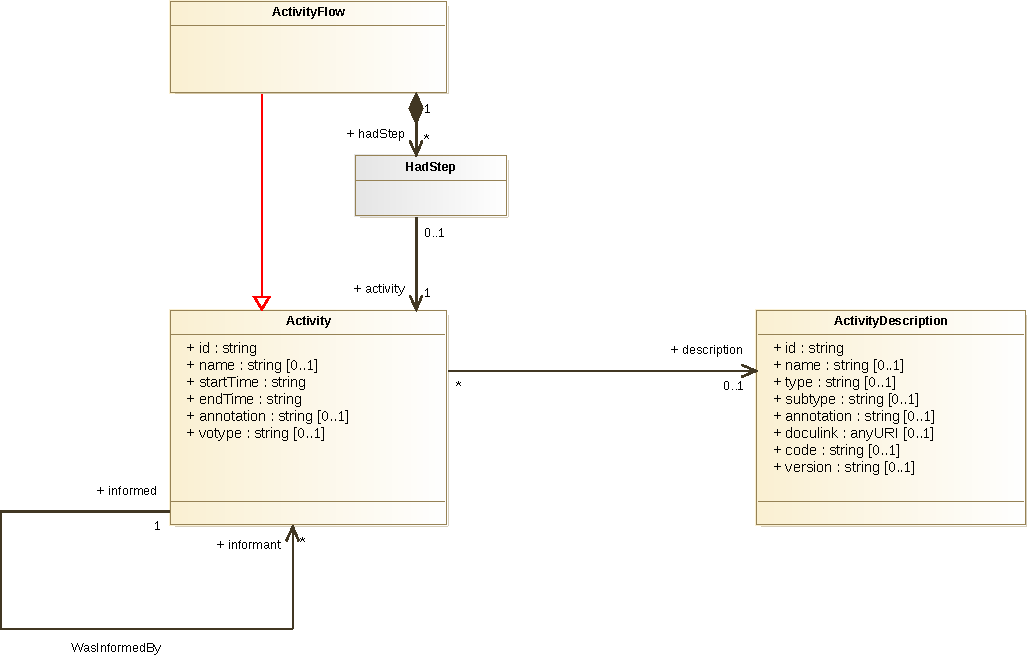
\includegraphics[scale=0.7]{activity-details.pdf}
%\caption[Details for Activity, ActivityDescription and ActivityFlow]{Details for Activity, %ActivityDescription and ActivityFlow (Sections~\ref{sec:activity} and \ref{sec:activityflow}).
%}
%\label{fig:activity-details}
%\end{figure}

\begin{table}[ht]
\small
\tymax  0.5\textwidth
\textbf{\normalsize Activity}\vspace{0.25em}\\
\begin{tabulary}{1.0\textwidth}{llLL}
\toprule
\head{Attribute} & \head{W3C PROV} & \head{Data type} & \head{Description}\\
\midrule
\textbf{id} & prov:id  & (qualified) string & a unique id for this activity (unique in its realm)\\
name        & prov:label  & string & a human-readable name (to be displayed by clients)\\
\textbf{startTime} & prov:startTime & datetime & start of an activity\\
\textbf{endTime} & prov:endTime  & datetime & end of an activity\\
% startTime and endTime are not strictly required -- and in case of a reproducible activity
% they are meaningless. Therefore, I removed the bf here.
% mireille :  I do not agree for this change by Ole : They can be unknown but they must be mandatory in order to allow to query on time for an activity, and to tell the execution order. 
annotation        & prov:description & string & additional explanations for the specific activity instance\\
status &  & string & can be used to describe the terminal status of the activity (e.g. completed, aborted, error...)\\
%votype & string & can be either ``activity'' or ``activityFlow''\\
%, used to differentiate between these two class types, if ``activityFlow'' is not implemented as an extra class (and in W3C compatible serializations)\\
%\midrule
%$\rightarrow$ description &  & link & link to \class{ActivityDescription}\\
%$\rightarrow$ wasAssociatedWith & prov:wasAssociatedWith  & link & link to \class{WasAssociatedWith} for linking with a responsible \class{Agent}\\
\bottomrule
\end{tabulary}
\caption[Attributes of \class{Activity}.]{Attributes of \class{Activity}, their data types and equivalents in the W3C PROV-DM, if existing. Attributes in bold are \textbf{mandatory}.}\label{tab:activity}
%, references are indicated with an arrow ($\rightarrow$).}
\end{table}


Activities in astronomy include all steps from obtaining data to the reduction
of  images and production of new datasets, such as image calibration, bias
subtraction, image stacking, light curve generation from a number of
observations, radial velocity determination from spectra, post-processing steps
of simulations, etc.

An Activity can be seen as the node that helps to discover the progenitors of a dataset and any additional information on its generation.

\paragraph{WasInformedBy.}
The individual steps of a pipeline can be chained together directly, without
mentioning the intermediate datasets, using the \class{WasInformedBy} relation.
This relation can be used as a shortcut if the skipped datasets are deemed
to be not important enough to be recorded. 
%For grouping activities, also see the next Section~\ref{sec:activityflow}.
It can also be used to state that an activity communicates with another through an output-input relation, and thereby triggers its execution (ProvONE specification).

\begin{table}[ht]
\small
\tymax  0.5\textwidth
\textbf{\normalsize WasInformedBy}\vspace{0.25em}\\
\begin{tabulary}{1.0\textwidth}{llL}
\toprule
\head{Attribute} & \head{Data type}   & \head{Description}\\
\midrule
\textbf{id} & string & an identifier for this relation\\
\midrule
%id               & string            & a unique id\\
$\rightarrow$ \textbf{informed} & link      & link to the \class{Activity} being informed by another (``second'' activity)\\
$\rightarrow$ \textbf{informant}      & link      & link to the informing \class{Activity} (``first'' activity)\\
%activity         & string            & id of the generation \class{Activity}\\
%generation       & string            & id of the \class{WasGeneratedBy} relation\\
%usage            & string            & id of the \class{Used} relation\\
\bottomrule
\end{tabulary}
\caption[Attributes of the \class{WasInformedBy} relation]{Attributes of the \class{WasInformedBy} relation.}\label{tab:wasinformedby}
\end{table}

% \paragraph{WasPartOf.}
% This relation, taken form the ProvONE ontology, enables the specification of the structure of \class{Activity} instances in that a parent \class{Activity} has child \class{Activities}. Such a structure can help to describe the steps of a pipeline, or a workflow.

% \begin{table}[ht]
% \small
% \tymax  0.5\textwidth
% \textbf{\normalsize WasPartOf}\vspace{0.25em}\\
% \begin{tabulary}{1.0\textwidth}{@{}lp{3cm}L@{}}
% \toprule
% \head{Attribute} & \head{Data type}   & \head{Description}\\
% \midrule
% %id               & string            & a unique id\\
% $\rightarrow$ \textbf{parent} & link      & link to the parent \class{Activity}, e.g. a workflow\\
% $\rightarrow$ \textbf{child}      & link      & link to the child \class{Activity}\\
% %activity         & string            & id of the generation \class{Activity}\\
% %generation       & string            & id of the \class{WasGeneratedBy} relation\\
% %usage            & string            & id of the \class{Used} relation\\
% \bottomrule
% \end{tabulary}
% \caption[Attributes of the \class{WasPartOf} relation]{Attributes of the \class{WasPartOf} relation.
% }\label{tab:waspartof}
% \end{table}


\subsubsection{Entity-Activity relations}
\label{sec:entity-activity-relations}

\begin{figure}[ht]
\centering
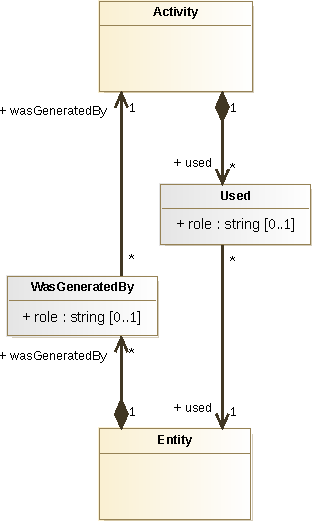
\includegraphics[scale=0.7]{entity-activity-relations-nodesc.pdf}
\caption[\class{Entity}-\class{Activity} relations]{\class{Entity} and \class{Activity} are linked via the \class{Used} and \class{WasGeneratedBy} relations. The \attribute{role} that an entity played when being used or generated by an activity is recorded  within the \class{Used} and \class{WasGeneratedBy} classes.}
\label{fig:entity-activity-relations}
\end{figure}

For each data flow it should be possible to clearly identify entities and 
activities. 
%If the activities shall not be recorded explicitely, one could also 
%use the \emph{Derivation}-relation as suggested in the W3C Provenance DM
%to link derived entities to their originals.
Each entity is usually a result from an activity, expressed by a link from 
the entity to its generating activity using the \class{WasGeneratedBy} relation,
and can be used as input for (many) other activities, expressed by the \class{Used} relation.
Thus the information on whether data is used as input or was produced as output of 
some activity is given by the \emph{relations} between activities and entities.
%In fact, 
%it would be enough to provide this information just for the relations on the description side (right).
% -- Is this true?

We use two relations, \class{Used} and \class{WasGeneratedBy} (see Tables~\ref{tab:used} and \ref{tab:wasgeneratedby}), instead of just one mapping class with a flag for input/output, because their descriptions and \attribute{role} attributes can be different. The \attribute{role} should always be provided if it is not obvious.
%in order to model the different 
%multiplicities explicitely: an entity always has only one (or none) 
%\class{WasGeneratedBy} relation, but may be \class{Used} many times as input for 
%different activities.


\begin{table}[ht]
\small
\tymax  0.5\textwidth
\textbf{\normalsize Used}\vspace{0.25em}\\
\begin{tabulary}{1.0\textwidth}{lllL}
\toprule
\head{Attribute} & \head{W3C PROV} & \head{Data type} & \head{Description}\\
\midrule
\textbf{id} & prov:id  & string & an identifier for this relation\\
role & prov:role & string   & role of the entity, defines as what it is being used\\
time & prov:time & datetime & time at which the usage of an entity started\\
\midrule
%\multicolumn{4}{@{}l}{References}\\
%\midrule
$\rightarrow$ \textbf{activity} & prov:activity & link & link to an \class{Activity}\\
$\rightarrow$ \textbf{entity} & prov:entity & link & link to an \class{Entity}\\
%$\rightarrow$ description  &  & link & link to the corresponding \class{UsedDescription}, if existing\\
\bottomrule
\end{tabulary}
\caption[Attributes and references of \class{Used} relation class]{Attributes and references of \class{Used} relation class. Attributes/references in bold are \textbf{mandatory}, references to other classes are indicated with an arrow ($\rightarrow$).}
\label{tab:used}
\end{table}

\begin{table}[ht]
\small
\tymax  0.5\textwidth
\textbf{\normalsize WasGeneratedBy}\vspace{0.25em}\\
\begin{tabulary}{1.0\textwidth}{lllL}
\toprule
\head{Attribute} & \head{W3C PROV} & \head{Data type} & \head{Description}\\
\midrule
\textbf{id} & prov:id  & string & an identifier for this relation\\
role & prov:role & string   & role of the entity that is generated by an activity, defines which output type it is\\
time & prov:time & datetime & time at which the generation of an entity is finished\\
\midrule
%\multicolumn{4}{@{}l}{References}\\
%\midrule
$\rightarrow$ \textbf{entity} & prov:entity & link & link to an \class{Entity}\\
$\rightarrow$ \textbf{activity} & prov:activity & link & link to an \class{Activity}\\
%$\rightarrow$ description  &  & link & link to the corresponding \class{WasGeneratedByDescription}, if existing\\
\bottomrule
\end{tabulary}
\caption[Attributes and references of \class{WasGeneratedBy} relation class]{Attributes and references of \class{WasGeneratedBy} relation class. Attributes/references in bold are \textbf{mandatory}, references to other classes are indicated with an arrow ($\rightarrow$).}
\label{tab:wasgeneratedby}
\end{table}


The \class{Used} and \class{WasGeneratedBy} relations can have the optional
attribute \attribute{time} -- this is the time when usage of an entity started
or the generation of an entity is finished.
%This generation time corresponds to e.g. \emph{DataID.date} in 
%Dataset Metadata DM.
%It therefore corresponds to the \emph{created}-time used in 
%the Simulation DM (SimDM). 

% 2018-09 commented
%\paragraph{Compositions and multiplicities}
%In principle, an entity is produced by just one activity.
%However, by introducing the \class{ActivityFlow} class for grouping activities together, 
%one entity can now have many wasGeneratedBy-links to activities. One of them must 
%be the actual generation activity, the other activities can only be activityFlows 
%containing this generation-activity. This restriction of having only one ``true'' generation activity is not explicitly expressed in the current model\footnote{The reason for this is that we want to keep the model simple and avoid introducing even more classes.}.


The \class{Used} relation is closely coupled to the \class{Activity}, so we use a composition here, indicated
in Figure~\ref{fig:entity-activity-relations} by a filled diamond: 
if an activity is deleted, then the corresponding used relations need to be removed as well. 
%mireille the appropriate figure with the diamonds is infact the original one from Kristin. we should refer to it 
The entities that were used still remain, since they may have been used for other activities as well.
We need a multiplicity * between \class{Used} and \class{Entity}, because an entity can be used more than once
(by different activities).

Similarly, the \class{WasGeneratedBy} relation is closely coupled with the \class{Entity} via a composition,
since a wasGeneratedBy relation makes no sense without its entity. So if an entity is deleted, 
then its wasGeneratedBy relation must be deleted as well. There is a multiplicity * between \class{Activity}
and \class{WasGeneratedBy}, because an activity can generate many entities.



\paragraph{Entity roles}\label{sec:entity-roles}
Each activity generally requires specific roles for each input or output entity.
% 2018-09 commented
%thus we store this information with description classes, in the role-attributes for the \class{UsedDescription} and \class{WasGeneratedByDescription} relation (see Tables~\ref{tab:useddescription} and \ref{tab:wasgeneratedbydescription}).
For example, an activity for dark-frame subtraction requires two input images. But it is 
very important to know which of the images is the raw image and 
which one fulfils the role of dark frame.

The role cannot be an attribute for \class{Entity}, 
since the same entity (e.g. a specific FITS file containing an image) may play 
different roles with different activities. If this is not the case, if the 
image can only play the same role everywhere, only then it is an intrinsic 
property of the entity.

%Additionally, input (and also output) data can take different roles in an 
%activity. For example, one file could
%be a parameter file, another one is the raw image, and the third one is the 
%dark field that should be subtracted. Since these roles are very important, 
%it must be made explicit which data component needs to fulfill which role as 
%input in or output from an activity.
%Each activity requires specific roles for each input or output entity, thus 
%we store this information on the description side, in the role-attributes for 
%the \class{UsedDescription} and \class{WasGeneratedByDescription} relation.

%In W3C, this is partially solved by adding a derivation relation between the Entities (data). Here, we have a mapping-class between Activity and DataEntities as well as between ActivityDescription and DataDescription. The mapping-class at the description side, i.e. between the ActivityDescription and its DataEntityDescriptions, contains additionally a role for each relation, e.g. parameter, dark frame, raw image, etc.  If a dataset is used as input to an activity or if it results from it, will become clear with these roles.

%Some example roles are given in Table \ref{tab:entity-roles}.
Note that these roles don't have to be unique, many datasets may play the same role for 
a process. For example, many image entities may be used as science-ready-images for an 
image stacking process. In order to facilitate interoperability, the possible entity-roles could be defined and described for each activity by the IVOA community, in a vocabulary list or thesaurus.

% \begin{table}[ht]
% \centering
% \small
% \begin{tabulary}{1.0\textwidth}{@{}lL@{}}
% \toprule
% \head{Role} & \head{Example entities}\\
% \midrule
% %configuration & configuration file \\ %& used for entities that contain configuration details for an activity\\
% %auxiliary input & calibration image, dark frame, etc. \\%& \\
% main input & raw image, science-ready images \\%& used for entities that are the main input for an activity\\
% main result & image, cube or spectrum \\%& used for entities that are the main result of an activity\\
% log & logging output file \\%& used for logging output \\
% red & image used for red channel of a composite activity\\%& used for images that will be used as the red channel of a composite activity\\
% \bottomrule
% \end{tabulary}
% \caption[Examples for entity roles]{Examples for entity roles}
% \label{tab:entity-roles}
% \end{table}
% % here we cross some notions encountered in parameter descriptions and Activity descriptions while describing parameters 


%\TODO{Roles can be used for checking (validation) if processes use the correct type of entities, 
%e.g. check if entity-type matches used-role!}

%Without the mapping tables, the relation between \class{Activity} 
%(\class{ActivityDescription}) and \class{Entity} (\class{EntityDescription})
%would be an aggregation relation, or in other words: an association with the 
%aggregation kind ``shared''. That would be required to ensure that all 
%entities linked to an activity (either as input or output) will survive if 
%the activity is destroyed, since they are almost always shared with other 
%activities. 
%
%By using the mapping tables we make the role of an entity in an activity more 
%explicit and thus can replace the aggregation by a composition relation to the 
%\class{Activity}/\class{ActivityDescription} and simple associations to the 
%individual data components and their descriptions. 


% The derivation relation together with entities is already enough to produce a 
% Data flow view, but in astronomy we are probably even more interested in the 
% Processes (as discussed in our first draft for requirements for provenance).

%\TODO{Add an example here! (From discussions in Heidelberg.)}





\subsubsection{Agent}\label{sec:w3c-agent}

An \class{Agent} describes someone who is responsible for a certain task or
entity, e.g. who pressed a button, 
ran a script, performed the observation or published a dataset.
The agent can be a single person, a group of persons, a 
project or an institute. 
This is also reflected in the IVOA Dataset Metadata Model, where \class{Party} 
represents an agent, and it has two types: \class{Individual} and \class{Organization},
which are explained in more detail in Table \ref{tab:agent-types} (also see Section~\ref{sec:dmlinks} for comparison between \class{Agent} and \class{Party}).
Both agent types are also used in the W3C PROV-DM, though 
\class{Individual} is called \class{Person} there.
%We decided to not include the type \class{SoftwareAgent} from W3C (yet), since it is not required for our current use cases. This may change in the future.

\begin{table}[ht]
\small
\tymax  0.5\textwidth
\textbf{\normalsize Agent}\vspace{0.25em}\\
\begin{tabulary}{1.0\textwidth}{lllL}
\toprule
\head{Attribute} & \head{W3C PROV} & \head{Data type} & \head{Description}\\
\midrule
\textbf{id} & prov:id & (qualified) string & unique identifier for an agent\\
\textbf{name} & prov:name & string & a common name for this agent; e.g. first name and last name; project name, agency name...\\
type & prov:type & string & type of the agent as given in Table~\ref{tab:agent-types}\\
email   &  & string & Contact email of the agent\\
affiliation   &  & string & Affiliation of the agent\\
address &  & string & Address of the agent\\
phone &  & string & Phone number\\
% insert here the attributes dedicated to contact for a Party in DataSet Metadata DM.
% \hline
% \multicolumn{4}{l}{Additional optional attributes from Dataset.Party subclasses:}\\
% \hline
% address &  & string & Address of the agent both for Individual (Person) and Organization\\
% phone   &  & string & Contact phone number of the agent both for Individual (Person) and Organization\\
% email   &  & string & Contact email of the agent both for Individual (Person) and Organization\\
\bottomrule
\end{tabulary}
\caption[\class{Agent} attributes]{\class{Agent} attributes}
\label{tab:agent}
\end{table}

\begin{table}[ht]
\small
\tymax  0.5\textwidth
\textbf{\normalsize AgentType}\vspace{0.25em}\\
\begin{tabulary}{1.0\textwidth}{lllL}
\toprule
\head{Class or type} & \head{W3C PROV} & \head{DatasetDM} &\head{Comment} \\
\midrule
Agent       & Agent  & Party & \\
Individual  & Person & Individual & a person, specified by name, email, address, 
      (though all these parts may change in time)\\
Organization & Organization & Organization & a publishing house, institute or scientific project\\
SoftwareAgent & & SoftwareAgent & A software agent is running software, e.g. a cron job or a trigger \\
\bottomrule
\end{tabulary}
\caption[Agent class and types of agents/subclasses]{Agent class and types of agents/subclasses in this data model, compared to W3C PROV-DM and Dataset DM.}
\label{tab:agent-types}
\end{table}

A definition of organizations is given in the 
IVOA Recommendation on Resource Metadata \citep{std:ResourceMeta}, hereafter 
referred to as RM: ``An organization is [a] specific type of resource that 
brings people together to pursue participation in VO applications.''
It also specifies further that scientific projects can be considered 
as organizations on a finer level:
``At a high level, an organization could be a university, observatory, or government
agency. At a finer level, it could be a specific scientific project, space mission,
or individual researcher. A provider is an organization that makes data and/or services
available to users over the network.''

For each agent a \attribute{name} must be specified. A summary of the attributes for \class{Agent} is given in Table~\ref{tab:agent}.
We added the optional attributes \attribute{address} and \attribute{email}, since they appeared in our use cases and are commonly used.
Not every project will need them; e.g. an advanced system may use permanent identifiers (e.g. ORCIDs, identities in federations, etc) to identify agents and retrieve their properties from an external system instead.
It would also increase the value of the given information if the (current) affiliation of the agent (and a project leader/group leader) were specified in order to maximize the chance of finding any contact person later on. 

\paragraph{Association and Attribution.}
The contact information is needed in case more information about a certain step in the past of a dataset is required, but also in order to know who was involved and to fulfil our ``Attribution'' requirement (Section~\ref{sec:requirements}), so that proper credits are given to the right people/projects. 

It is desired to have at least one agent given for each activity (and entity), but it
is not enforced.
% , hence the multiplicity between \class{Entity}/\class{Activity} and the relations
%to the \class{Agent} starts with 0.
There can also be more than one agent for each activity/entity with different \attribute{roles} and one agent can be responsible for more than one activity or entity. This many-to-many relationship is made explicit in our model by adding the two following relation classes: 
\class{wasAssociatedWith}, that relates an \class{Activity} to an agent, and
\class{wasAttributedTo}, that relates an \class{Entity} to an agent.

We adopted here the same naming scheme that was used in the W3C PROV-DM.
Note that the attributed-to-agent for a dataset may be different from the 
agent that is associated with the activity that created an entity.
Someone who is performing a task is not necessarily given full attribution, 
especially if he acts on behalf of someone else (the project, university, ...).


\begin{table}[ht]
\small
\tymax  0.5\textwidth
\textbf{\normalsize WasAssociatedWith}\vspace{0.25em}\\
\begin{tabulary}{1.0\textwidth}{lllL}
\toprule
\head{Attribute} & \head{W3C PROV} & \head{Data type} & \head{Description}\\
\midrule
\textbf{id} & prov:id  & string & an identifier for this relation\\
role & prov:role & string   & role of the agent, see e.g. Table~\ref{tab:agent-roles}\\
\midrule
%\multicolumn{4}{@{}l}{References}\\
%\midrule
$\rightarrow$ \textbf{agent} & prov:agent & link & link to an \class{Agent}\\
$\rightarrow$ \textbf{activity} & prov:activity & link & link to an \class{Activity}\\
%$\rightarrow$ description  &  & link & link to the corresponding \class{WasGeneratedByDescription}, if existing\\
\bottomrule
\end{tabulary}
\caption[Attributes and references of \class{WasAssociatedWith} relation class]{Attributes and references of \class{WasAssociatedWith} relation class. Attributes/references in bold are \textbf{mandatory}, references to other classes are indicated with an arrow ($\rightarrow$).}
\label{tab:wasassociatedwith}
\end{table}


\begin{table}[ht]
\small
\tymax  0.5\textwidth
\textbf{\normalsize WasAttributedTo}\vspace{0.25em}\\
\begin{tabulary}{1.0\textwidth}{lllL}
\toprule
\head{Attribute} & \head{W3C PROV} & \head{Data type} & \head{Description}\\
\midrule
\textbf{id} & prov:id  & string & an identifier for this relation\\
role & prov:role & string   & role of the agent, see e.g. Table~\ref{tab:agent-roles}\\
\midrule
%\multicolumn{4}{@{}l}{References}\\
%\midrule
$\rightarrow$ \textbf{agent} & prov:agent & link & link to an \class{Agent}\\
$\rightarrow$ \textbf{entity} & prov:entity & link & link to an \class{Entity}\\
\bottomrule
\end{tabulary}
\caption[Attributes and references of \class{WasAttributedTo} relation class]{Attributes and references of \class{WasAttributedTo} relation class. Attributes/references in bold are \textbf{mandatory}, references to other classes are indicated with an arrow ($\rightarrow$).}
\label{tab:wasattributedto}
\end{table}


%\TODO{\textbf{Mireille + Fran\c{c}ois}: Go through these roles, pick only the necessary ones, crosscheck with other data models.}

In order to make it clearer what an agent is useful for, we suggest the
possible roles an agent can have (along with descriptions partially taken from RM)
in Table~\ref{tab:agent-roles}.
For comparison, SimDM, the IVOA Simulation DM \citep{std:SimDM} contains following roles for their contacts:
owner, creator, publisher and contributor. Note that the \emph{Party} class in Dataset and SimDM are very similar to the \emph{Agent} class, which is explained in more detail in the appendix, Section~\ref{sec:dmlinks}.

This list is \emph{not} complete. We consider providing a vocabulary list for this in a future version of this model, collected from (future) implementations of this model.


\begin{table}[ht]
\small
\tymax  0.5\textwidth
\textbf{\normalsize AgentRoles}\vspace{0.25em}\\
\begin{tabulary}{1.0\textwidth}{llL}
\toprule
\head{role} & \head{type or sub class} & \head{Comment} \\
\midrule
author & Individual & someone who wrote an article, software, proposal\\
contributor & Individual & someone who contributed to something (but not enough to gain authorship)\\
editor & Individual & editor of e.g. an article, before publishing\\
creator & Individual & someone who created a dataset, creators of articles or software are rather called ``author''\\
curator & Individual & someone who checked and corrected a dataset before publishing\\
publisher & Organization & organization (publishing house, institute) that published something\\
observer & Individual & observer at the telescope\\
operator & Individual & someone performing a given task \\ % removed executor: ambiguous
coordinator & Individual & someone coordinating/leading a project\\ % we should choose one word : PI?
funder & Organization & agency or sponsor for a project as in PROV-N\\
provider & Organization & ``an organization that makes data and/or services available to users over the network'' (definition from RM)\\
%(owner) & voprov:Individual or voprov:Organization & Does anyone really own the data?\\
\bottomrule
\end{tabulary}
\caption[Examples for roles of agents]{Examples for roles of agents and the typical type of that agent}
\label{tab:agent-roles}
\end{table}


%\TODO{Do we have a specific use case for fixing the agent-roles? Is anyone 
%going to search for specific roles in the Provenance meta-data?
%Or shall we leave it open, which roles can be defined and just give examples here?}
% ... Yes, just give examples here. Should have a vocabulary list somewhere ...

%\subsubsection{Shortcuts: WasDerivedFrom and WasInformedBy}\label{sec:shortcuts}
%The classes \class{WasDerivedFrom} and \class{WasInformedBy} can be used as ``shortcuts'' and 
%are used in the same way as the corresponding W3C classes.

%\class{WasDerivedFrom} defines the relation that links two entities together, if one entity was derived
%from the other entity. In principle, one can find this information also by tracing the 
%history of an entity backwards to the generating activity and its input entities. 
%The descriptions for activity, entity and their relations should provide enough
%information to find the progenitor entity from which an entity was derived.
%Nevertheless, we include \class{WasDerivedFrom} for those cases where an explicite 
%link between an entity and its progenitor is useful (e.g. for speeding up searches for 
%progenitors or if the activity in between is not important).

%The class \class{WasInformedBy} links two activities together without defining the
%intermediate entities that may have been exchanged. This is useful for e.g. pipelines, 
%if the intermediate entities don't play a major role or only exist temporarily, so that
%their provenance information is not deemed to be important enough to be recorded.
%``WasInformedBy'' relation (also called ``Communication'' relation, borrowed from W3C's model) 






\clearpage

\subsection{Extended Model}
\label{sec:extended_model}


\subsubsection{Class diagram and VO-DML compatibility}
\label{sec:extended_model_diagram_vodml}

\begin{figure}[ht]
\centering
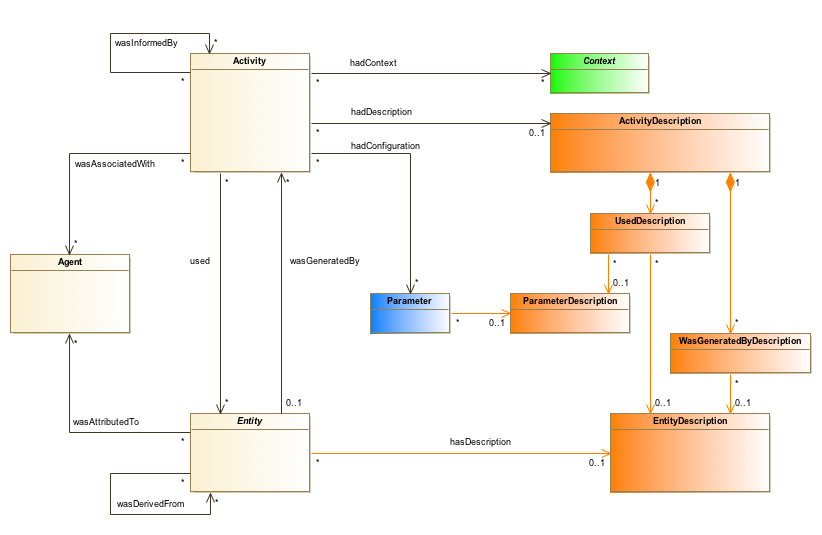
\includegraphics[width=1.0\textwidth]{ExtendedModel.png}
\caption[Class diagram showing the main functional features of the Provenance DM]{Class diagram showing the main functional features of the Provenance DM. This diagram includes a subset of all the specialized entities and relations defined in this section. Those are presented in separate diagrams and in the text.}
\label{fig:classdiagram}
\end{figure}

\begin{figure}[ht]
\centering
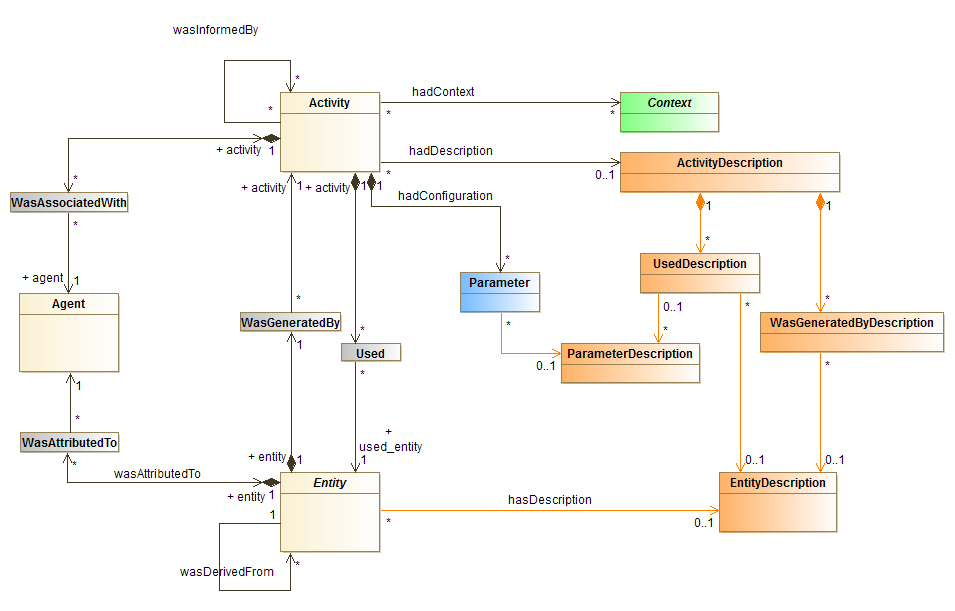
\includegraphics[width=1.0\textwidth]{ExtendedModel_VODML.png}
\caption[VO-DML compatible version of the class diagram in Figure~\ref{fig:classdiagram}]{VO-DML compatible version of the class diagram in Figure~\ref{fig:classdiagram}.}
\label{fig:classdiagram_vodml}
\end{figure}

In the domain of astronomy, certain processes and steps are repeated over and over again, maybe using a different configuration and within a different context. 
We therefore separate the descriptions of activities from the actual processes and introduce an additional \class{ActivityDescription} class. 
Likewise, we also apply the same pattern for \class{Entity} and add an \class{EntityDescription} class. Defining such descriptions allows them to be reused, which is less redundant when performing a series of tasks of the same type. 
A similar normalization of descriptions of the actual processes and datasets can be found in the IVOA Simulation DM \citep[SimDM, ][]{std:SimDM}), which describes simulation metadata. The SimDM classes \class{Experiment} and \class{Protocol} correspond to the Provenance terms \class{Activity} and \class{ActivityDescription}.

Figure~\ref{fig:classdiagram} shows the global class diagram. In addition to the core model (Section~\ref{sec:core_model}), we define specialized entities (Section\ref{sec:spec_entities}) and relations (Section\ref{sec:spec_relations}) that were identified as useful in one or several use cases. 
For some of the concepts that are well known in the IVOA ecosystem, we propose a detailed structure in order to facilitate the access to such resources and foster interoperability (Sections~\ref{sec:entity_desc}, \ref{sec:parameters} and \ref{sec:activity_desc}).

% 1018-09 commented
% %The association
% %classes for the many-to-many relations are modelled as mapping classes.
% When implementing the model in a relational database, the many-to-many relations can be
% represented as individual tables for mapping the relation. We model one of each
% of the associations of the many-to-many relationships as a composition (full
% diamond) if the mapping class belongs more strongly to one of its linked
% classes; e.g. the \emph{Used} relations are strongly dependent on the
% corresponding \emph{Activities}. 

Figure~\ref{fig:classdiagram_vodml} shows a version of the UML diagram that is fully VO-DML compliant, i.e. we just used the restricted subset of UML to model Provenance and reused the IVOA datatypes.
%In order to be compliant to VO-DML (see Section~\ref{sec:extended_model_diagram_vodml}), 
In addition to the modification presented in Figure~\ref{fig:classdiagram_vodml}, we model the membership relation explicitly by including a \class{HadMember} class in our model, which is connected to the\class{Collection} class via a composition.


The documentation of all classes and an automatically generated figure based on the underlying xmi-description behind this UML diagram is available in the Volute repository at
\url{https://volute.g-vo.org/svn/trunk/projects/dm/provenance/vo-dml/ProvenanceDM.html}.


%\begin{table}[ht]
%\small
%\tymax  0.5\textwidth
%\begin{tabulary}{1.0\textwidth}{@{}lp{3cm}lp{3cm}L@{}}
%\toprule
%\head{IVOA Aspects} & \head{Construct type} & \head{Name} & \head{Specification} \\
%\midrule
%\multirow{6}{*}{Entity Structure} & \multirow{6}{*}{Class} & Entity & Section~\ref{}\\
% & & Collection & Section~\ref{}\\
% & & Data & Section~\ref{}\\
% & & Visualization & Section~\ref{}\\
% & & Document & Section~\ref{}\\
% & & Device & Section~\ref{}\\
%\midrule
%
%\bottomrule
%\end{tabulary}
%\caption[IVOA Provenance DM constructs]{IVOA Provenance DM constructs}
%\label{tab:constructs}
%\end{table}


 
\subsubsection{Specialized Entities}
\label{sec:spec_entities}

The abstraction level of the W3C PROV-DM being high, one of the objective of this IVOA recommendation is to guide the usage of this model in the astronomy context by providing specialized entities that are connected to concepts known in astronomy and relevant to assess the quality and reliability of the exchanged entities.

We first remind the W3C PROV definition of an \class{Entity}: ‘‘An entity is a physical, digital, conceptual, or other kind of thing with some fixed aspects; entities may be real or imaginary.''

We already expressed the necessity of adding \textbf{Descriptions} to the concepts of Activity and Entity, in order to avoid redundancy and give detail explanations on the method or algorithms that compose the core of an activity. In addition, from our use cases in Astronomy, activities require specific metadata that is related to the \textbf{Configuration} of an activity, the \textbf{Context}. We therefore define  specialized entities hierarchically following those main categories. The structuring links of specialized entities is presented in Figure~\ref{fig:spec_entities}. The list given below is not intended to be exhaustive, additional project-dependant entities may be defined when relevant.

\begin{figure}[ht]
\centering
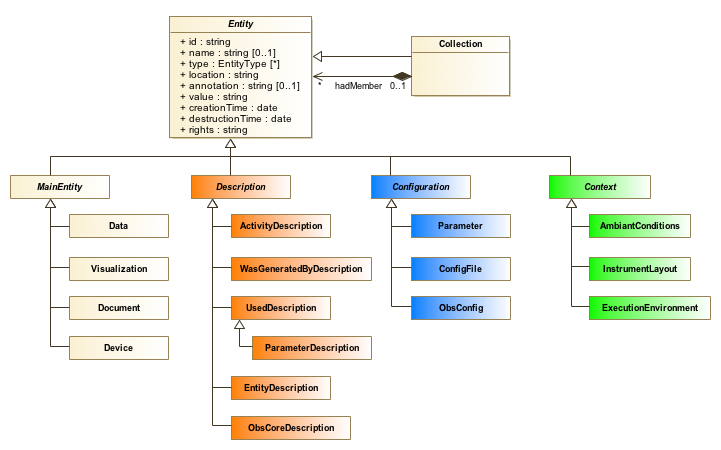
\includegraphics[width=1.0\textwidth]{SpecializedEntities.png}
\caption{Class diagram showing the structuring links for specialized entities}
\label{fig:spec_entities}
\end{figure}

It is important to note that specialized entities inherit from \class{Entity}, all those classes thus share the identifier attribute  \attribute{id}, as well as the relations of the core model. The \attribute{id} attribute must be unique for each different entity so that it can be connected to other concepts using core or specialized relations (see Section~\ref{sec:spec_relations}). It is possible to attach an Agent to any of those subclasses of \class{Entity} in order to provide specific contacts for the content of a specialized entity.

\paragraph{MainEntity:}
Provenance information are expected to be recorded primarily for those main entities, to which we may attach descriptions, detail the configuration that led to their generation and the context in which they were generated. 
\begin{itemize}
\item[\textbf{Data}]: digital, machine-readable information in some content that will be used/transformed/analysed. It could be a cell or a column in a table, a file, an image, a cube of data... This \class{Data} \class{Entity} might be bounded to a IVOA \class{Dataset} record.
\item[\textbf{Visualization}]: a digital visual representation.
\item[\textbf{Document}]: information presented in a human readable form, e.g. a book, an article, or an observation proposal.
\item[\textbf{Device}]: a physical object, such as a tool, an instrument, a telescope, etc.
\end{itemize}
We note that \class{Data}, \class{Visualization} and \class{Document} are classes that are also defined in the ProvONE ontology \citep{ProvONE}, with the following text: ''The \class{Data} class is defined to be generic and represents data items of various types (e.g. XML, JSON, CSV files, etc.). \class{Visualizations} are a differentiated class intended to represent various visualization items often output from workflows (JPG, PNG, SVG, MP4, etc.). The \class{Document} class is a generic representation of a published or unpublished article or report.‘‘

\paragraph{Description:}
This subclass of entities carries detailed information on the expected behaviour of an \class{Activity} and on the expected structure and use of an \class{Entity}. It describes in a structured way the plan prepared for and followed by an activity, and as such, influences directly the activity.
\begin{itemize}
\item[\textbf{ActivityDescription}]: explanations on the activity, such as the method used, the algorithm, the source code. This class is further described in Section~\ref{sec:activity_desc}.
\item[\textbf{ParameterDescription}]: contains the attributes of a \class{Parameter} that are similar to the attributes of the PARAM block in a VOTable (unit, UCD, UType...). This class is further described in Section~\ref{sec:parameters}.
\item[\textbf{UsedDescription}]: describes the roles of expected inputs in an Activity, e.g. a red channel in the creation of an RGB image.
\item[\textbf{WasGeneratedByDescription}]: describes the roles of expected outputs in an Activity, e.g. a master bias in the stacking of a set of bias images.
\item[\textbf{EntityDescription}]: describes a category of entities, and contains descriptive information about an entity that is known before an entity instance is created (file format, MIME or content type, etc), for example: all files that follow the FITS-LDAC structure and format in a project. This class is further described in Sections~\ref{sec:entity_desc} and \ref{sec:activity_desc}.
\item[\textbf{ObsCoreDescription}]: contains the IVOA ObsCore fields that can be attached to an entity, e.g. in the case of a released dataset.
\end{itemize}

\paragraph{Configuration:}
This subclass of entities corresponds to the information passed to an activity in order to configure its , and it thus directly influences the development of an activity.
\begin{itemize}
\item[\textbf{Parameter}]: configuration of the activity before execution as a key=value parameter in the IVOA framework, e.g. the number of bins desired in the sampling of a signal. This class is further described in Section~\ref{sec:parameters}.
\item[\textbf{ConfigFile}]: file containing configuration information for the activity, e.g. a list of parameters (key=value) for a script, generally in a given format (txt, json, xml, yaml...)
\item[\textbf{ObsConfig}]: structured list of parameters that gives the configuration of an observation. For example this can point to specific observing modes of an instrument, the filters used, the trigger mode, etc.
\end{itemize}

\paragraph{Context:}
This subclass of entities gives more information on the context that influences  the development of an activity, but for which there are no or little control at the moment of its execution:
\begin{itemize}
\item[\textbf{AmbientConditions}]: common, prevailing, and uncontrolled atmospheric and weather conditions in a room or place that influence the activity.
\item[\textbf{InstrumentLayout}]: description of how the instrument is structured and how the hardware is set up at the beginning of an activity.
\item[\textbf{ExecutionEnvironment}]: describes a particular execution platform, such as an operating system or a database management system. Execution environments are used to describe the context in which the execution of an activity takes place. Execution environments could also describe the computing hardware of a system.
\end{itemize}



\subsubsection{Specialized Relations}
\label{sec:spec_relations}

In order to distinguish the different specialized entities in their usage or influence, we define the corresponding specialized relations between \class{Activity} and \class{Entity}: \class{hadDescription}, \class{hadConfiguration} and \class{hadContext}, that should be connected to the entity categories \class{Description}, \class{Configuration} and \class{Context}, respectively. An \class{Activity} should have one or zero \class{Description} element of type \class{ActivityDescription}. In addition, we introduce the \class{hasDescription} relation between two \class{Entity} classes. Those relations are illustrated in Figure~\ref{fig:spec_relations}.

\begin{figure}[ht]
\centering
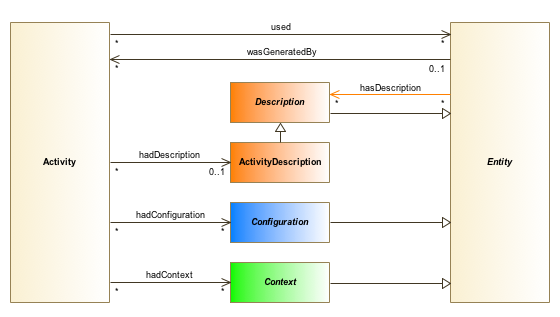
\includegraphics[width=1.0\textwidth]{figures/SpecializedRelations.png}
\caption{Class diagram showing the relations between specialized entities and \class{Activity} or \class{Entity}}
\label{fig:spec_relations}
\end{figure}

We thus provide a way to qualify the usage or influence of a specialized entity on an activity, or another entity. The \attribute{role} attribute in those relations is not expected to be defined as they are already qualified and generally point to specialized entities. Those relations can thus be seen as simple association tables.


\subsubsection{EntityDescription}
\label{sec:entity_desc}

\begin{table}[ht]
\small
\tymax  0.5\textwidth
\textbf{\normalsize EntityDescription}\vspace{0.25em}\\
\begin{tabulary}{\textwidth}{llL}
\toprule
\head{Attribute} & \head{Data type} & \head{Description}\\
\midrule
\textbf{id} & (qualified) string & a unique identifier for this description\\
name       & string & a human-readable name for the entity description\\
annotation  & string & a decriptive text for this kind of entity\\
%category    & string & specifies if the entity contains information on logging, system (environment), calibration, simulation, observation, configuration, ...\\
doculink    & url & link to more documentation\\
\midrule
\multicolumn{3}{@{}l}{\textbf{Optional attributes:}} \\
content\_type    & string & MIME type for the content of the entity\\
format    & string & type of container for the entity\\
% removed the obscore attributes, since specific for observations only, not applicable to configuration entities etc.
% dataproduct\_ type  & string       & from ObsCore data model \citep{std:ObsCore}, if applicable; describes, what kind of product it is (e.g. image, table)\\
% dataproduct\_ subtype & string       & from ObsCore data model, more specific subtype\\
% level       & enum integer & the level of processing or calibration; for ObsCore's calib\_level it is an integer between 0 and 3\\
%\midrule
%\multicolumn{4}{@{}l}{\textbf{Additional attributes:}} \\
%\multicolumn{4}{@{}l}{Further project-specific attributes (e.g. format, content\_type) and/or attributes}\\
%\multicolumn{4}{@{}l}{from other data models (e.g. dataproduct\_type and -\_subtype, version, calibLevel}\\
%\multicolumn{4}{@{}l}{from DatasetDM) can be added (Section~\ref{sec:dataset-obscore}).}\\
\bottomrule
\end{tabulary}
\caption[Attributes of \class{EntityDescription}]{Attributes of \class{EntityDescription}. 
%For simple use cases, this description class may be ignored and its attributes may be used for \class{Entity} instead.
%The utypes may vary depending on the data model, e.g. for simulation data they 
%would point to utypes of SimDM.
}\label{tab:entitydescription}
\end{table}


%The Entity class can have an EntityDescription class attached. 
The types of entities can be predefined using a
description class \class{EntityDescription}. This class is meant to store
descriptive information % In English,'information' lacks a plural form.
about an entity that is known before an \class{Entity} instance is created.
For example, if we run an activity to create an RGB image from three greyscale
images, we may know a mandatory \attribute{format} for the input and output
images before the activity's execution (JPG, PNG, FITS, \ldots), but we probably
cannot know the final \attribute{size} of the image  that will be created.
In this example, \attribute{format} would be an \class{EntityDescription} attribute,
while \attribute{size} would be an attribute of the \class{Entity} instance. 
The \class{EntityDescription} general attributes are summarized in Table 
\ref{tab:entitydescription}.

%This class thus stores entity-related 
Additional attributes that describe the content of the data could be derived from 
the Dataset Metadata Model (see Section \ref{sec:dataset-obscore})

The \class{EntityDescription} class should \emph{not} contain information about the usage of the data, in particular, it tells nothing about them being used as
input or as output. This kind of information should be provided by the
relations (and their relation descriptions) between activities and entities
(see Section \ref{sec:entity-activity-relations}).




\subsubsection{Parameter and ParameterDescription}
\label{sec:parameters}

\begin{table}[b]
\small
\tymax  0.5\textwidth
\textbf{\normalsize Parameter}\vspace{0.25em}\\
\begin{tabulary}{1.0\textwidth}{llL}
\toprule
\head{Attribute} &  \head{Data type} & \head{Description}\\
\midrule
\textbf{id}      & string & parameter unique identifier\\
%description\_ref   & foreign key/url & link to \emph{ParameterDescription}\\
%name            & string & parameter name, if no link to ParameterDescription is given\\
\textbf{value}   & (value dependent) & the value of the parameter, type depends on \attribute{ParameterDescription.datatype} and \attribute{xtype}; follows same rules as VOTable TABLEDATA and DALI\\ % TODO: check and put proper reference somewhere!
\midrule
%$\rightarrow$ activity & link & link to \class{Activity}\\
$\rightarrow$ description & link & link to \class{ParameterDescription}\\
\bottomrule
\end{tabulary}
\caption[Attributes of \class{Parameter}]{Attributes of \class{Parameter}. Attributes in bold are \textbf{mandatory}, references to other classes are indicated with an arrow ($\rightarrow$).}
\end{table}
\footnote{Attributes in bold are \textbf{mandatory}, references to other classes are indicated with an arrow ($\rightarrow$).}
\begin{table}[ht]
\small
\tymax  0.5\textwidth
\textbf{\normalsize ParameterDescription}\vspace{0.25em}\\
%\begin{tabulary}{1.0\textwidth}{@{}p{2.5cm}p{0cm}lL@{}}
\begin{tabulary}{1.0\textwidth}{p{2cm}lL}
\toprule
\head{Attribute} &  \head{Data type} & \head{Description}\\
\midrule
\textbf{id}  & string & parameter unique identifier\\
\textbf{name} & string & parameter name\\
annotation  & string & additional free text description\\
datatype    & string & datatype as in VOTable 1.2 and above \\
arraysize     & number & number of values of specified \attribute{datatype}, if there is more than one\\
unit           & string & physical unit \\
ucd           & string  & Unified Content Descriptor, supplying a standardized classification of the physical quantity\\
utype        & string  & Utype, meant to express the role of the parameter in the context of an external data model \\
xtype         & string & extended datatype as in VOTable 1.2 and above\\
\midrule
\multicolumn{3}{@{}l}{\textbf{Optional attributes:}} \\
min           & number & minimum value \\
max           & number & maximum value\\
options     & list & list of accepted values\\
value       & (value dependent) & the default value of the parameter, type depends on \attribute{datatype} and \attribute{xtype}; follows same rules as VOTable TABLEDATA and DALI\\
\midrule
$\rightarrow$ activityDescription & link & link to \class{ActivityDescription}\\
\bottomrule
\end{tabulary}
\caption[Attributes of \class{ParameterDescription}]{Attributes of \class{ParameterDescription}.}
\end{table}

The concept of activity configuration, generally a set of parameters that can be configured before the execution of an activity, is tightly linked to the concept of provenance. Configuration information can indeed be relevant to assess the quality and reliability of an activity or an entity.

Activity configuration typically implies a set of parameters attached to the activity before execution. The concept of parameter is very general, and already exists in the VO context, for example as PARAM elements in VOTable \citep{std:VOTABLE}, as uws:param elements in the UWS pattern \citep{std:UWS}, or as POST/GET parameters for web services \citep[see for example][]{std:SODA}. The Simulation DM also contains a ParameterSetting class \citep{std:SimDM}.

%We identify three different ways to link configuration information to an activity:
%\begin{itemize}
%\item Declare a parameter set (or each parameter) as an input entity that is used by the activity. \\
%        This also allows tracking the provenance of the parameter further.
%\item Define families of activities, each one with fixed attributes.\\
%        I.e. use different subclasses for activities with different fixed attributes.
%\item Add activity attributes in the form of key-value parameters.
%\end{itemize}

In order to provide a link between configuration and provenance information, we add a \class{Parameter} class along with a \class{ParameterDescription}, so that configuration information is structured and stored with the provenance information (and can thus be queried simultaneously). 

%The \class{Parameter} class is an entity that should be connected to an activity with the specialized usage relation hadConfiguration. 
The optional attributes of \class{ParameterDescription} are taken from the FIELD and PARAM elements in VOTable \citep{std:VOTABLE}. 
%The \attribute{value} attribute should provide the default value proposed for a parameter.

% 2018-09 commented
%We note that a parameter can be seen as a simplified entity, though it can only be used by an activity and it has no provenance. In some cases, it may be relevant to define a specific parameter as an entity if its provenance should be traced.

%For example, observations generally require information on \emph{ambient conditions} as well as 
%\emph{instrument characteristics}. This contextual data associated with an observation is not directly modelled in the ProvenanceDM. However, this information can be stored as different entities. 
%Alternatively, one could list the instrument characteristics as a set of key-value parameters using the \class{Parameter} class, so that this information is structured and stored with the provenance information (and can thus be queried simultaneously). 

For example, in the case of a processing activity that cleans an image with a sigma-clipping method, the input and output images would be entities and the value of the number of sigma for sigma-clipping would be carried by a \class{Parameter} entity. The corresponding \class{ParameterDescription} would define the type and range of the expected value for this parameter (using the attributes datatype, min, max, options...).
%We may also want to define a 3-sigma-clipping activity where this parameter is fixed to 3.


%For example for observations, the \emph{ambient conditions} as well as 
%\emph{instrument characteristics} need to be stored. But they can both be treated
%as additional entities as well. 
%Our model can then also take into account that a certain observation
%method requires special ambient conditions, already defined via the 
%ActivityDescription (e.g. radio observations rely on different ambient 
%conditions than observations
%of gamma rays), just following our data -- data description scheme.
%Ambient conditions are recorded for a certain time (startTime, endTime) and are
%usually only valid for a certain time interval. This time interval should be recorded
%with a \emph{validity}-attribute for such entities.
%
%In contrast to ambient conditions, instrument characteristics do (usually) not
%change from one observation to the other, so they are static, strictly related to
%the instrument. 
%All the characteristics could be described either as key-value pairs directly with the 
%observation (as attributes) or just as datasets, using the \class{Entity} class. 
%One would then 
%link the instrument characteristics as a type of input (or output?) dataset to a certain 
%observation activity. Thus we don't need a separate Instrument or Device class.

%\note{One should also keep in mind that some instrument related parameters can change within time,
%e.g. the CCD temperature. The instruments can also change within time because of aging.}

\paragraph{Parameter value vs. Entity value.}
A parameter \attribute{value} can be derived from an entity \attribute{value} (its content or part of its content), thus having itself an origin, with provenance information.
The \attribute{value} of a parameter can sometimes be an identifier, a file name, or a URL (e.g. of datatype string) that points to an entity (e.g. a dataset). However, the parameter does not transport the value (or content) of the referenced entity. It is thus not clear if the parameter value points to an input or output entity, or if it is just a string. To remove this ambiguity, one could describe the used or generated entity in the UsedDescription or WasGeneratedByDescription classes presented in the next section, using the same name as the parameter. This would indicate that an entity is connected to an activity by simply giving its identifier through a parameter. In that case, the \attribute{ucd} of the parameter as given in the \class{ParameterDescription} should indicate that this is an identifier (e.g. \attribute{meta.id}). The associated \attribute{utype} would then point to \attribute{Entity.id}.
% I don't understand the chapter above: Since a Parameter is an Entity, it may have a 
% \attribute{value} or a \attribute{location}, depending on whether it is the value itself or
% a reference. Why would you put an URL into the \attribute{value} field then?
% If we split the ParameterDescription into an EntityDescription and a UsedDescription, then
% there is no need to specify \attribute{utype} in case of references at all. And we can use
% ucds & Co. in entity related values that are no parameters.

\paragraph{Parameter value vs. ParameterDescription value.}
The \class{ParameterDescription} class being a child of the \class{Entity} class, it contains a \attribute{value} attribute. As this Description class contains information known before a \class{Parameter} instance is created (as for EntityDescription in Section~\ref{sec:entity_desc}), its value can be considered to be the default value expected for the parameter.



\subsubsection{Activity Description classes}
\label{sec:activity_desc}


\begin{table}[ht]
\small
\tymax  0.5\textwidth
\textbf{\normalsize ActivityDescription}\vspace{0.25em}\\
\begin{tabulary}{1.0\textwidth}{llL}
\toprule
\head{Attribute} &  \head{Data type} & \head{Description}\\
\midrule
\textbf{id}  & string & a unique id for this activity description (unique in its realm)\\
name         & string & a human-readable name (to be displayed by clients)\\
location    &  string & a path or a URL to the ActivityDescription serialization\\
annotation  & string & additional free text description for the activity\\
doculink     & url    & link to further documentation on this activity, e.g. a 
paper, the source code in a version control system etc.\\
\midrule
\multicolumn{3}{@{}l}{\textbf{Optional attributes:}} \\
group        & string & type of the activity, from a vocabulary or list, e.g. data acquisition (observation or simulation), reduction, calibration, publication\\
subgroup     & string & more specific subtype of the activity\\
code         & string & the code (software) used for this process, if applicable\\
version      & string & a version number, if applicable (e.g. for the code)\\
\bottomrule
\end{tabulary}
\caption[Attributes of \class{ActivityDescription}]{Attributes of \class{ActivityDescription}. Some of the attributes inherited from Entity (see Table~\ref{tab:entity}) are not indicated in this table.}
\end{table}


The plan or method underlying an activity can be specified by a corresponding \class{ActivityDescription} class. This could be, for instance, the name of the \attribute{code} and its \attribute{version} used to perform an activity or a more general description of the underlying algorithm or process. 
An activity is then a concrete case (instance) of using such a plan or method, with a \attribute{startTime} and an \attribute{endTime}, and it refers to a corresponding description for further information.

A close concept in the W3C PROV-DM is the \class{Plan} (also defined as a subclass of \class{Entity}), however a plan in PROV-DM is attached to an \class{Agent} with \class{hadPlan} through the \class{wasAssociatedWith} relation, while \class{ActivityDescription} is directly attached to \class{Activity} and can thus be seen as an additional list of attributes that describes the \class{Activity} that are known before an \class{Activity} instance is created. If an \class{Agent} is associated to an \class{Activity} and responsible for its execution, the \class{ActivityDescription} concept becomes fully compatible with the W3C PROV \class{Plan} concept.

There MUST be exactly zero or one \class{ActivityDescription} per \class{Activity}. If steps from a pipeline shall be grouped together, one needs to create a proper 
\class{ActivityDescription} for describing all the steps at once. This method can then 
be referred to by the pipeline activity. 

\paragraph{Descriptions of the Used and WasGeneratedBy relations}
In order to describe more largely an activity, it is common to define the expected inputs and outputs of this activity, i.e. what we expect to store in the Used and WasGeneratedBy relations.

In the case of workflow descriptions, such as ProvONE (but also Kepler or Taverna for example), input and output \textbf{ports} are defined, and can be connected to build a workflow of activities. In ProvONE \citep{ProvONE}, an \class{ActivityDescription} is restricted to a \class{Program}, and an \class{Activity} is an \class{Execution} associated to a \class{Program}, with further entities and relations dedicated to workflow descriptions (see Section\ref{sec:dmlinks}). However, the description of workflows is out of the scope of this document, and the more general concepts we introduce here are the UsedDescription and the WasGeneratedByDescription classes. Those classes are meant to store descriptive information about the usage or generation of an entity that is known before the activity is executed.

In particular, if the \attribute{role} attribute is given in those description classes, the corresponding \class{Used} and \class{WasGeneratedBy} relations must contain the same \attribute{role} value. The \attribute{multiplicity} attribute indicates that more than one entity may have the same role, e.g. in the case of the stacking of several images, all the input images share the exact same role.

%When serializing the DM, the attributes of the description class may be assigned to the activity for simplification.
% in order to produce  a W3C compliant serialization, which is the same procedure as with
% Entity\slash{}EntityDescription).


\begin{table}[ht]
\small
\tymax  0.5\textwidth
\textbf{\normalsize UsedDescription}\vspace{0.25em}\\
\begin{tabulary}{1.0\textwidth}{llL}
\toprule
\head{Attribute} &  \head{Data type} & \head{Description}\\
\midrule
\textbf{id} & string & identifier\\
role & string   & entity role; defines the role of an entity, as what it is used for the linked type of activityDescription\\
\midrule
\multicolumn{3}{@{}l}{\textbf{Optional attributes:}} \\
multiplicity & string & Number of expected input entities to be used with the given role. The multiplicity is 1 by default and a * indicates an unknown or unlimited number of input entities.\\
\midrule
$\rightarrow$ \textbf{activityDescription} & link & link to \class{ActivityDescription}\\
$\rightarrow$ entityDescription & link & link to \class{EntityDescription}\\
\bottomrule
\end{tabulary}
\caption[Attributes and references of \class{UsedDescription} class]{Attributes and references of \class{UsedDescription} class. Attributes/references in bold are \textbf{mandatory}, references to other classes are indicated with an arrow ($\rightarrow$).}
\label{tab:useddescription}
\end{table}


\begin{table}[ht]
\small
\tymax  0.5\textwidth
\textbf{\normalsize WasGeneratedByDescription}\vspace{0.25em}\\
\begin{tabulary}{1.0\textwidth}{llL}
\toprule
\head{Attribute} & \head{Data type} & \head{Description}\\
\midrule
\textbf{id} & string & identifier\\
role & string & entity role; defines the role of an entityDescription, which kind of output it is\\
\midrule
\multicolumn{3}{@{}l}{\textbf{Optional attributes:}} \\
multiplicity & string & Number of expected output entities that will be generated with the given role. The multiplicity is 1 by default and a * indicates an unknown or unlimited number of input entities.\\
\midrule
$\rightarrow$ \textbf{activityDescription} & link & link to an \class{ActivityDescription}\\
$\rightarrow$ entityDescription & link & link to \class{EntityDescription}\\
\bottomrule
\end{tabulary}
\caption[Attributes and references of \class{WasGeneratedByDescription} class]{Attributes and references of \class{WasGeneratedByDescription} class. Attributes/references in bold are \textbf{mandatory}, references to other classes are indicated with an arrow ($\rightarrow$). }
\label{tab:wasgeneratedbydescription}
\end{table}

\paragraph{Input parameters.}
\class{ParameterDescription} can be seen as a specialized input port attached to an \class{ActivityDescription}. We thus expect a list of parameters for an activity, described with the attributes listed in Section~\ref{sec:parameters}. This \class{ParameterDescription} is not expected to have a \attribute{role} attribute, however the \attribute{name} attribute should correspond to its \attribute{role}. Such a list of input parameters already exist in the IVOA ecosystem for service resources, in this context, they are written in the form of an IVOA DataLink Service Descriptor \citep{std:Datalink}.

\paragraph{EntityDescription in the context of an Activity.}
%The description of the different ports is completed by the description of the  type of entity accepted as an input or output of the activity.
When related to the \class{UsedDescription} or \class{WasGeneratedByDescription}, the attributes of EntityDescription (see Section~\ref{sec:entity_desc}) help to describe the category of entities expected as an input or an output in an activity. For example: the input bias files must be in FITS format, or the red, green and blue channel images must be in PNG or JPEG format. 
